\section{Monday, October 30, 2019}

\subsection{Insertion in Binary Search Trees}

Last class, we described how we can search for an element in a binary search tree: making comparisons at each step tells us whether we should make a recursive subcall on the left or right subtree. Following a similar procedure, we can easily insert values into binary search trees. Suppose we have the following binary search tree:

\begin{figure}[h]
\centering
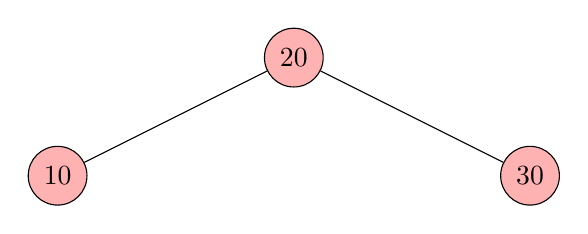
\begin{tikzpicture}[level/.style={sibling distance=60mm/#1}]
\node [circle,draw,fill=red!30] (z){$20$}
  child {node [circle,draw,fill=red!30] (a) {$10$}
    % child {node [circle,draw,fill=red!30] (b) {$2$}
    % }
    % child {node [circle,draw,fill=red!30] (g) {$4$}}
  }
  child {node [circle,draw,fill=red!30] (j) {$30$}
};
\end{tikzpicture}
\caption{A Binary Search Tree}
\end{figure}

Suppose we want to insert the value $35$. We start off by making a comparison with the root node ($20$), and we determine that the value $35$ belongs in the right subtree of $20$. Next, we make a comparison with $30$, and we determine that the value $35$ belongs in the right subtree of $30$. But since $30$ has no right subtree, we stop recursing, and we add the value $35$ where it belongs. A newly inserted value will \textbf{always} end up as a leaf node in the new tree.  Similar to searching, we note that insertion requires $\O(\log(n))$ time in the average case, but it takes $\O(n)$ time in the worst case (when the tree is degenerate). 

What's an example in which the worst case behavior is exhibited? Suppose we insert a sequence of values in ascending or descending order. This will surely result in a degenerate tree, and our tree's insertion method will operate similar to a Linked List's insertion method. This is bad since we will end up performing in $\O(n)$ time rather than $\O(\log(n))$ time. 

\subsection{Deletion in Binary Search Trees}

So far, insertion and searching in binary search trees has just involved starting at the root node, and recursing on the left or right subtree, depending on what a comparison yields. However, deleting a node in a binary search tree can be a little bit trickier. 


The general outline for deleting a node $X$ in a binary search tree is described below:
\begin{enumerate}
    \item Perform a search for value $X$ in the binary search tree.
    \item If $X$ is a leaf node, delete $X$.
    \item Otherwise, $X$ must be an internal node. In this case, replace $X$ with the largest value $Y$ on the left subtree or the smallest value $Z$ on the right subtree. Now recursively call this delete method on the replacement value (either $Y$ or $Z$) from the subtree.
\end{enumerate}

The reason why deletion in a binary search tree might seem complicated is that we must preserve the binary search tree property when we are removing a node from the tree. The method described above ensures that we do not violate the binary search tree property even after a node has been removed. Our base case here is deleting a leaf node since our binary search tree property can never be violated if we just remove a leaf. 

\subsection{Binary Search Tree Implementation}

So far, we've mostly discussed the theory behind trees and binary search trees. But how do we actually implement a binary search tree in Java? In order to do this, we need to create a class that represents a Binary Search Tree, and this class needs to have an inner class representing a node inside of a binary search tree (this is very similar to how we implemented a Linked List).

Here's one way in which we can begin the implementation of a generic binary search tree:

\begin{lstlisting}
public class BinarySearchTree <K extends Comparable<K>, V> {
    private class Node {
        private K key;
        private V data;
        private Node left, right;
    }
    
    public Node(K key, V data) {
        this.key = key;
        this.data = data;
    }
}
\end{lstlisting}

Note that our we require the generic type \verb!K! to extend \verb!Comparable! since our binary search tree property imposes an ordering on its elements. Each node has a reference to its left and right subtree. The \verb!key! entry in the \verb!Node! class represents the quantity that we are using to determine the node's relative order to the other nodes in the tree. On the other hand, the \verb!data! field represents the actual data that the node is storing (in some cases, these two quantities might be the same). 

Here is an implementation of the \verb!add! method which incorporates the ideas that we have already discussed:

\begin{lstlisting}
	public boolean add(K key, V data) {
		if (root == null) {
			root = new Node(key, data);
			return true;
		} else {
			return addAux(key, data, root);
		}
	}

	private boolean addAux(K key, V data, Node rootAux) {
		int comparison = key.compareTo(rootAux.key);

		if (comparison == 0) {
			rootAux.data = data;
			return false;
		} else if (comparison < 0) {
			if (rootAux.left == null) {
				rootAux.left = new Node(key, data);
				return true;
			} else {
				return addAux(key, data, rootAux.left);
			}
		} else {
			if (rootAux.right == null) {
				rootAux.right = new Node(key, data);
				return true;
			} else {
				return addAux(key, data, rootAux.right);
			}
		}
	}
\end{lstlisting}

Firstly, in the \verb!add! function, we check whether \verb!root! is null. If it is, our tree is currently empty, which means that we just need to make the node that we are adding equal to the root. On the other hand, if we enter the \verb!else { ... }! clause, our tree is non-empty, and we must make use of our recursive auxillary function. In the auxillary function, we compare the value that we wish to add with the node that we are currently at. If the two values are equal, we just update the data (and do not add a new node). On the other hand, if the value we are adding is less than the current node we are at, we either add the node as the left child of the current node (if there is no left child), or we recurse on the left subtree. The case in which the comparison yields that the value we are adding has a key larger than the current node's key is similar, except we recurse and add onto the right subtree. 


Next, we'll discuss an implementation of a \verb!toString()! method, which prints the values in a binary search tree:

\begin{lstlisting}
    	public String toString() {
		return toStringAux(root);
	}

	private String toStringAux(Node rootAux) {
		return rootAux == null ? ""
				: toStringAux(rootAux.left) + "{" + rootAux.key + ":" + rootAux.data + "}" + toStringAux(rootAux.right);
	}
\end{lstlisting}

This method is fairly short. We use a recursive helper function \verb!toStringAux()! to perform an in-order traversal on our tree. We check whether the current root we are at is null (in this case, there is nothing to print). If it isn't null, we print the data associated with the left subtree followed by the data associated with the current node, and we finally print all of the data in the right subtree. As we mentioned before, an in-order traversal prints the values in a binary search tree in ascending order of the node's keys.

Finally, here is an implementation of a \verb!find! method, which returns true provided that an inputted node exists in the binary search tree:

\begin{lstlisting}
      public boolean find(K key) {
		return find(key, root);
	}

	public boolean find(K key, Node rootAux) {
		if (rootAux == null) {
			return false;
		} else {
			int comparison = key.compareTo(rootAux.key);
			if (comparison == 0) {
				return true;
			} else if (comparison < 0) {
				return find(key, rootAux.left);
			} else {
				return find(key, rootAux.right);
			}
		}

\end{lstlisting}

This implementation is very similar to the insertion method. We make comparisons at each step, which allows us to easily target where the value should be present in the binary search tree (if it exists at all). 